\chapter{WCDMA 移动通信系统}
\section{WCDMA 系统概述}
三种方案对比,详细见书P186。
\subsection{WCMDA的发展}
GSM->GPRS->EDGE->WCDMA->HSDPA->HSUPA>LET\\
详细演进版本可见P187。
\subsection{WCMDA系统结构}
无线接入 网负责处理所有与无线通信相关的
功能。而 CN 则采用了 GSM/GPRS 的定义,这样可
以实现网络的平滑过渡,核心网负责对话音及
数据业务进行交换和路由查找,以便将业务连
接至外部 网络.
\begin{figure}[H]
	\centering
	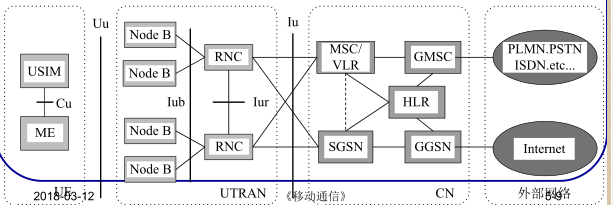
\includegraphics[width=0.7\linewidth]{figures/screenshot011}
	\caption{}
	\label{fig:screenshot011}
\end{figure}
\begin{enumerate}
	\item UE,UE 完成人与网络间的交互,通过\textbf{ Uu 接口}与无
	线接入网相连,与网络进行信令和数据交换。包
	括两部分:
	\begin{itemize}
		\item ME,移动设备
		\item USIM,UTMS用户识别模块。
	\end{itemize}
	\item 无线接入网(UTRAN),UTRAN 位于两个开放接口 Uu 和 Iu 之间,完成所有
	与无线有关的功能。
	\begin{itemize}
		\item 无线网络控制器( RNC ),主要完成连接建立和断开、切换、宏分集合并
		和\textbf{无线资源管理控制}等功能。
		\begin{enumerate}
			\item 控制 RNC ( CRNC )。对于某个 Node B 来说,直接
			控制它的 RNC 就是\textbf{控制} RNC ( CRNC )
			\item 服务 RNC(SRNC) 。与 CN 有连接,为 UE 提供资源的
			RNC。(越区切换合并)
			\item 漂移 RNC(DRNC) 。把自己的资源借给 SRNC 为某一
			个 UE 使用的(仅一个Node B资源)
		\end{enumerate}
		\begin{figure}[H]
			\centering
			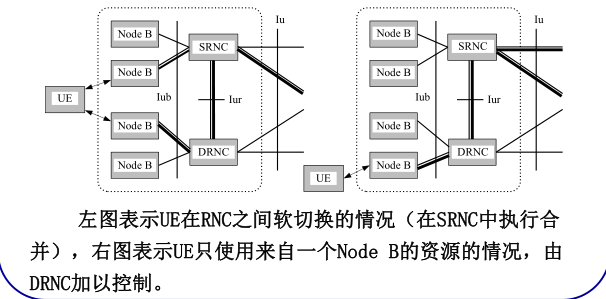
\includegraphics[width=0.7\linewidth]{figures/screenshot012}
			\caption{}
			\label{fig:screenshot012}
		\end{figure}
		\item Node B,Node B 通过 Iub 接口和基站控制器 RNC 互连。它主
		要由接口电路、基带处理单元、射频前端和控制单元
		部分组成。\textbf{ Node B=BBU(基带处理)+RRU(射频前端+ 天馈系统},\textbf{基带处理是核心功能},Node B 还负责完成更软切换、定位测量和执行无
		线资源分配与管理控制指令的功能
	\end{itemize}
	\item  CN 核心网络。
	\begin{itemize}
		\item CS域:MSC/VLR,GMSC
		\item PS域:SGSN,GGSN,CG。
		\item HLR.
	\end{itemize}
	\item 接口
	\begin{enumerate}
		\item Cu,USIM和ME之间
		\item Uu,UE和UTRAN,是UMTS中最重要的开放接口之一。
		\item Iu,UTRAN和CN。
		\item Iur,RNC之间
		\item Iub,Node B之间。
	\end{enumerate}
\end{enumerate}
\subsection{CDMA的优点}
\begin{enumerate}
	\item 抗干扰能力强,特别是抗窄带干扰;
	\item 可检测性低,不容易被侦破
	\item 具有多址能力,易于实现码分多址技术
	\item 可抗多径干扰
	\item 可抗频率选择性衰落
	\item 频谱利用率高,容量大
\end{enumerate}
\subsection{UTRAN 接口协议}
\subsubsection{结构图}
\begin{figure}[H]
	\centering
	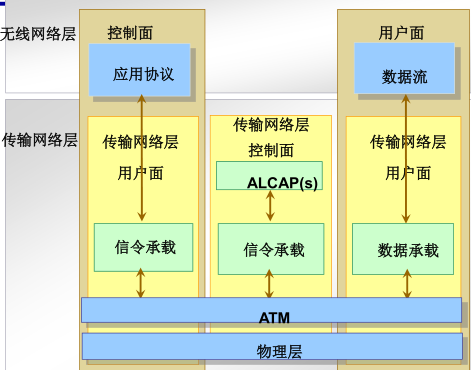
\includegraphics[width=0.7\linewidth]{figures/screenshot014}
	\caption{}
	\label{fig:screenshot014}
\end{figure}
特点:
\begin{enumerate}
	\item 所有接口具有开放性
	\item 将无线网络层与传输层分离
	\item 控制面和用户面分离
\end{enumerate}
Iu,Iub,Iur使用\textbf{ATM}承载。
\subsubsection{协议栈}
\textbf{UTRAN 控制面协议栈}是指协议和设备的对应关系
。 \textbf{UE 里面实现的协议是最完备}的,所有的 Node B 只实
现第一层,从 Uu 口的角度来讲,\textbf{ RNC 实现第二层(}从
MAC 到 RRC ),\textbf{ CN 只实现 RRC 之上的}
\begin{figure}
	\centering
	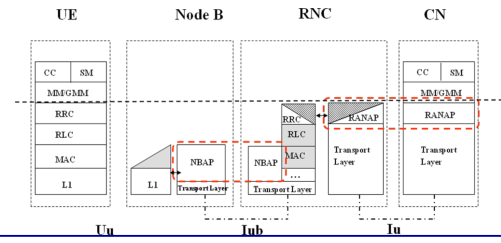
\includegraphics[width=0.7\linewidth]{figures/screenshot015}
	\caption{}
	\label{fig:screenshot015}
\end{figure}
UTRAN 用户面协议栈用户面有 CS 和 PS 域,从 UE的角度讲,没有RRC。
\begin{figure}
	\centering
	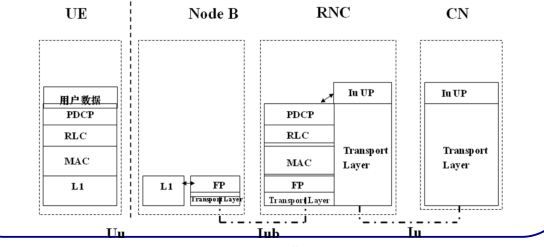
\includegraphics[width=0.7\linewidth]{figures/screenshot016}
	\caption{}
	\label{fig:screenshot016}
\end{figure}
\section{WCDMA系统的关键技术}
\subsection{基本技术}
WCDMA 系统发射机和接收机的信号处理流程
\begin{enumerate}
	\item 信源编码 。自适应多 速率 AMR
	技术( 带8 8 种信源 速率) .
	\item 信道编码 、交织,抵抗无线传播环境中的各种衰落。主要采用 卷积码、 Turbo 码和交
	织等信道编码技术
	\item 扩 频、加扰,这两步是 WCDMA 系统所特有的,采用高速的OVSF提高数
	字符号的速率,增加信号带宽
	\item 调制,
\end{enumerate}
\subsection{RAKE接收}
\begin{itemize}
	\item 多径分离
	\item 多径合并准则
	\item  RAKE接收的本质。
\end{itemize}
\subsection{功率 控制技术}
从通信链路的角度,功率控制可 分为
\begin{itemize}
	\item 前向功率控制,基站到移动台
	\item 反向功率控制,移动台到基站
\end{itemize}
从 功率控制方法的角度,功率控制可 分为
\begin{itemize}
	\item 开环功率控制
	\item 闭环功率控制
\end{itemize}
快速 、准确的\textbf{功率 控制技术}是 保证 WCDMA 系统性
能的\textbf{核心 }技术。
\subsubsection{反向开环功率控制}
根据接收到的钱箱链路信号的功率大小来调整自己的发射功率。开环功率控制由于补偿信道中的\textbf{平均路径损耗及慢衰落},有一个很大的\textbf{动态范围}。\\
开环功率控制只能起到粗略控制
的作用 。
\subsubsection{反向闭环 功率控制}
建立于开环功率控制之上,最开环功率控制进行校正。根据反向链路上移动台的信号强弱,产生功率控制指令,通过前向链路将功率指令发送给移动台,移动台根据该指令,在开环功率控制所选择发射功率的基础上,快速校正自己功率。克服\textbf{快衰落}。
\begin{itemize}
	\item 内环功率控制,基站测量移动台的移动台信号,与某个门限比较,进行发送相应的功率控制指令。
	\item 外环功率控制,对内环门限进行调整。
\end{itemize}
\subsection{软切换}










